% ch07b Local magnetic moments in metals, part b (书页 70-79 / 分册p020-029)
\section{Friedel求和规则与局域磁矩}

在推导局域磁矩形成的条件之前，先从传导电子被杂质散射的相移的角度看一看我们所得结果的结构，是有益的。利用式 (7.22)，我们发现传导电子的格林函数满足
\begin{equation*}
(\epsilon + \mathrm{i}\Gamma - \epsilon_{\mathbf{k}})G^{\sigma}_{\mathbf{k}\mathbf{k}'}(\epsilon + \mathrm{i}\Gamma) = \delta_{\mathbf{k}\mathbf{k}'} + V_{\mathbf{k}d}G^{\sigma}_{d\mathbf{k}'}(\epsilon + \mathrm{i}\Gamma).
\tag{7.101}
\end{equation*}
利用式 (7.24) 与式 (7.25) 消去 $G^{\sigma}_{\mathbf{k}d}$，便得到封闭表达式
\begin{equation*}
G^{\sigma}_{\mathbf{k}\mathbf{k}'}(\epsilon + \mathrm{i}\Gamma) = \frac{\delta_{\mathbf{k}\mathbf{k}'}}{\epsilon + \mathrm{i}\Gamma - \epsilon_{\mathbf{k}}} + \frac{V_{\mathbf{k}d}}{\epsilon + \mathrm{i}\Gamma - \epsilon_{\mathbf{k}}}G^{\sigma}_{dd}(\epsilon + \mathrm{i}\Gamma)\frac{V^{*}_{\mathbf{k}'d}}{\epsilon + \mathrm{i}\Gamma - \epsilon_{\mathbf{k}'}}.
\tag{7.102}
\end{equation*}
格林函数的这个表达式具有如下形式
\begin{equation*}
G = G_{0} + G_{0}TG_{0},
\tag{7.103}
\end{equation*}
其中 $T$ 是 $T$ 矩阵，
\begin{equation*}
T = V + VG_{0}T.
\tag{7.104}
\end{equation*}
于是，我们把动量 $\mathbf{k}$ 的传导电子散射到动量 $\mathbf{k}'$ 的 $T$ 矩阵确认为
\begin{equation*}
T^{\sigma}_{\mathbf{k}\mathbf{k}'}(\epsilon + \mathrm{i}\Gamma) = V_{\mathbf{k}d}G^{\sigma}_{dd}(\epsilon + \mathrm{i}\Gamma)V^{*}_{\mathbf{k}'d}.
\tag{7.105}
\end{equation*}
注意到，由于相互作用 $V_{\mathbf{k}d}$ 按假定与 $\mathbf{k}$ 的方向无关，散射只发生在 $s$ 波通道。代入式 (7.29)，我们得到
\begin{equation*}
T^{\sigma}_{\mathbf{k}\mathbf{k}}(\epsilon + \mathrm{i}\Gamma) = \frac{|V_{\mathbf{k}d}|^{2}}{\epsilon + \mathrm{i}\Gamma - E_{d\sigma} + \mathrm{i}\pi N(\epsilon)V|\bar{V}_{\mathbf{k}d}|^{2}},
\tag{7.106}
\end{equation*}
从而，$T$ 矩阵的虚部
\begin{equation*}
\mathrm{Im}T^{\sigma}_{\mathbf{k}\mathbf{k}}(\epsilon + \mathrm{i}\Gamma) = -\pi|V_{\mathbf{k}d}|^{2}\rho_{d\sigma}(\epsilon),
\tag{7.107}
\end{equation*}
正比于 $d$ 能级上的态密度。

由初等散射理论，
\begin{equation*}
T^{\sigma}_{\mathbf{k}\mathbf{k}'}(\epsilon + \mathrm{i}\Gamma) \propto \mathrm{e}^{2\mathrm{i}\delta_{\sigma}} - 1 \propto \sin\delta_{\sigma}\mathrm{e}^{\mathrm{i}\delta_{\sigma}} = 1/(\cot\delta_{\sigma} - \mathrm{i}).
\tag{7.108}
\end{equation*}
于是，我们把 $s$ 波相移确认为
\begin{equation*}
\cot\delta_{\sigma}(\epsilon) = \frac{E_{d\sigma} - \epsilon}{\Delta}.
\tag{7.109}
\end{equation*}

“在壳上”（on shell），即当 $\epsilon_{\mathbf{k}} = \epsilon_{\mathbf{k}'} = \epsilon$ 时，$T$ 矩阵元化为标准形式
\begin{equation*}
T^{\sigma}_{\mathbf{k}\mathbf{k}}(\epsilon + \mathrm{i}\Gamma) = -\frac{1}{\pi N(\epsilon)V}\sin\delta_{\sigma}\mathrm{e}^{\mathrm{i}\delta_{\sigma}}.
\tag{7.110}
\end{equation*}

如前所述，$d$ 能级的平均占据数 $\langle n_{d\sigma}\rangle$ 由态密度对被填充态的积分给出，
\begin{align*}
\langle n_{d\sigma}\rangle &= \int_{-\infty}^{\epsilon_{\mathrm{F}}=0}\rho_{d\sigma}(\epsilon)\,\mathrm{d}\epsilon \\
&= \frac{\Delta}{\pi}\int_{-\infty}^{0}\frac{\mathrm{d}\epsilon}{(\epsilon - E_{d\sigma})^{2} + \Delta^{2}} \\
&= \frac{1}{\pi}\cot^{-1}\left(\frac{E_{d\sigma}}{\Delta}\right).
\tag{7.111}
\end{align*}
利用式 (7.109)，我们得到
\begin{equation*}
\langle n_{d\sigma}\rangle = \frac{\delta_{\sigma}(0)}{\pi},
\tag{7.112}
\end{equation*}
这就是弗里德德尔求和规则的简化形式，它把杂质格点的占据数与在费米能处受杂质散射的传导电子的相移联系起来。我们强调，这里计算的相移完全来自 $d$ 能级上的无非自旋翻转散射。自旋翻转散射的作用将在下一章明确讨论近藤（Kondo）问题时予以强调。

将表达式 $E_{d\sigma} = \epsilon_{d} + U\langle n_{d-\sigma}\rangle$（译注：原文此处误印为 $E_d$，按式 (7.10) 应为 $\epsilon_d$）代入式 (7.111)，我们得到两个耦合方程，
\begin{equation*}
\langle n_{d\uparrow}\rangle = \frac{1}{\pi}\cot^{-1}\left(\frac{\epsilon_{d} + U\langle n_{d\downarrow}\rangle}{\Delta}\right)
\tag{7.113}
\end{equation*}
以及
\begin{equation*}
\langle n_{d\downarrow}\rangle = \frac{1}{\pi}\cot^{-1}\left(\frac{\epsilon_{d} + U\langle n_{d\uparrow}\rangle}{\Delta}\right),
\tag{7.114}
\end{equation*}
它们分别给出杂质 $\uparrow$ 与 $\downarrow$ 自旋能级的占据数。这就是安德森哈密顿量的哈特里–福克处理的核心方程。

为形成局域磁矩，我们寻找满足 $\langle n_{d\uparrow}\rangle \ne \langle n_{d\downarrow}\rangle$ 的解。只有在这种情形下 $d$ 杂质才是磁性的。首先，我们立即看到：若 $U = 0$，唯一的解是 $\langle n_{d\uparrow}\rangle = \langle n_{d\downarrow}\rangle$。而在 $\Delta \to \infty$ 的极限下，我们同样只能得到非磁解 $\langle n_{d\uparrow}\rangle = \langle n_{d\downarrow}\rangle = 1/2$。然而，在中间参数区域 $\Delta/U \ll 1$，存在磁化解。为简化记号，我们引入无量纲参数 $x = -\epsilon_{d}/U$ 与 $y = U/\Delta$。$x = 0$ 对应 $d$ 态能量 $\epsilon_{d}$ 恰好位于费米能级处。$x = 1$ 时，$\epsilon_{d} = -U$，能量为 $\epsilon_{d} + U$ 的上 $d$ 态与费米能级简并。因此，能量 $0$ 与 $-U$ 对称地分布在 $x = 1/2$ 即 $\epsilon_{d} = -U/2$ 的两侧。我们将看到，$x = 1/2$ 是磁矩形成最有利的情形。事实上，磁性仅在 $0 \le x \le 1$ 时得以保持。当 $\epsilon_{d} = -U/2$ 时，哈密顿量中的杂质项 $\sum_{\sigma}(\epsilon_{d}n_{d\sigma} + V_{\mathbf{k}d}a^{\dagger}_{d\sigma}a_{\mathbf{k}\sigma}) + Un_{d\uparrow}n_{d\downarrow}$ 在变换 $a_{d} \to a^{\dagger}_{d}$ 下具有粒子–空穴对称性（见习题 7.4）。

\begin{figure}[H]\centering
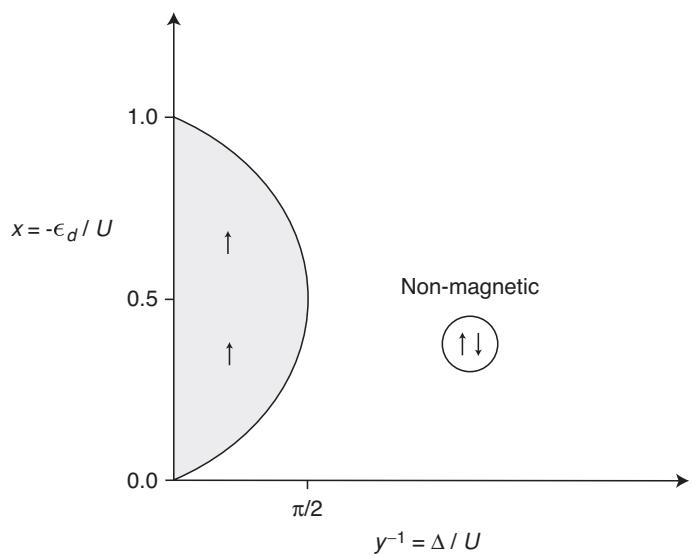
\includegraphics[width=0.58\textwidth]{figs/ch07/fig_7.3.jpg}
\caption*{图 7.3\quad 安德森模型的局域磁矩相图。在阴影区域内，局域磁矩稳定地形成。实线分隔磁性与非磁性区域。}\label{fig:auto:7.3}
\end{figure}

在 $y \gg 1$ 且 $1 > x > 0$ 的极限下，式 (7.113) 与式 (7.114) 预言如下形式的磁化解：
\begin{equation*}
\pi\langle n_{d\uparrow}\rangle \simeq \pi + \frac{1}{y(\langle n_{d\downarrow}\rangle - x)}
\tag{7.115}
\end{equation*}
以及
\begin{equation*}
\pi\langle n_{d\downarrow}\rangle \simeq \frac{1}{y(\langle n_{d\uparrow}\rangle - x)},
\tag{7.116}
\end{equation*}
其中 $\langle n_{d\uparrow}\rangle \sim 1$、$\langle n_{d\downarrow}\rangle \sim 0$。在 $y$ 大的极限下，解为
\begin{align*}
\langle n_{d\uparrow}\rangle &= 1 - \frac{1}{\pi xy} + \cdots, \\
\langle n_{d\downarrow}\rangle &= x + \frac{1}{\pi xy} + \cdots.
\tag{7.117}
\end{align*}

完整磁性参数范围的相图示于图 7.3。在转变曲线上及其外侧，$\langle n_{d\uparrow}\rangle = \langle n_{d\downarrow}\rangle \equiv n_{d}$，等价地，$\cot\pi n_{d} = (\epsilon_{d} + Un_{d})/\Delta$。混合价区域对应于相图的左下与左上区域，在那里下能级或上能级与费米能级近于简并。在这两个区域中的任何一个里，稍稍增大 $\Delta$ 都会得到非磁解。如前所述，许多电子体系——例如重费米子材料——正处于这一区域。在界定局域磁矩形成区域的边界上，对等占据概率 $n_{d} = n_{c}$（即 $\langle n_{\sigma}\rangle = n_{c} + \sigma\delta n$）施加无穷小微扰，就会导致杂质能级占据数的不相等。于是，由式 (7.113) 与式 (7.114)，我们直接发现：在相边界上，占据数必须同时也是局域磁矩方程的导数方程的解，即
\begin{equation*}
1 = \frac{U}{\Delta\pi}\frac{1}{1 + [(\epsilon_{d} + Un_{c})/\Delta]^{2}}.
\tag{7.118}
\end{equation*}

\begin{figure}[H]\centering
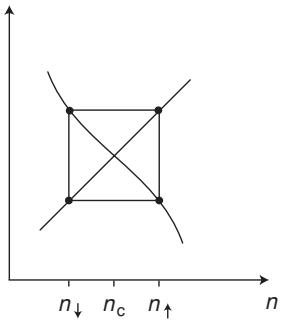
\includegraphics[width=0.42\textwidth]{figs/ch07/fig_7.4.jpg}
\caption*{图 7.4\quad 曲线 $y(n - x)$ 与 $\cot\pi n$ 交点处的图示。围绕交点所作矩形的顶点对应式 (7.113) 与式 (7.114) 的磁解。}\label{fig:auto:7.4}
\end{figure}

推导相边界这一形式的等价方式，是考察曲线 $\cot\pi n$ 与 $y(n - x)$ 交点附近的解，如图 7.4 所示。式 (7.113) 与式 (7.114) 的解可以用围绕这类交点、形如图 7.4 所示的矩形来描述：当 $\langle n_{d\uparrow}\rangle > \langle n_{d\downarrow}\rangle$ 时，矩形的右边竖边位于 $\langle n_{d\uparrow}\rangle$ 处，左边竖边位于 $\langle n_{d\downarrow}\rangle$ 处，如图所示。只要矩形的各个顶点都触到曲线，磁解就能存在。在 $\cot\pi n = y(n - x)$ 的交点附近作无穷小偏移时，若两条曲线 $\cot\pi n$ 与 $y(n - x)$ 的斜率大小相等、符号相反，则得到磁解。这正是式 (7.118) 给出的条件。

将式 (7.118) 与式 (7.30) 加以比较即可看出，磁性稳定性条件等价于
\begin{equation*}
U\rho_{d}(\epsilon = 0) = U\rho_{d}(\epsilon_{\mathrm{F}}) = 1,
\tag{7.119}
\end{equation*}
其中等占据时 $\rho_{d}(\epsilon) = \rho_{d\uparrow}(\epsilon)\,(=\rho_{d\downarrow}(\epsilon))$。这个方程是安德森局域磁矩理论的主要结果。在费米能级处态密度大的磁性杂质，预期会在非磁性金属中形成局域磁矩。事实上，注意到局域磁矩的形成在杂质能级半满时最为有利（见图 7.3），我们可以更直观地看出局域磁矩判据。半满时，局域磁矩判据即式 (7.118) 化为 $U/\pi\Delta > 1$。杂化能量通过 $\Delta$ 由跳跃矩阵元的平方决定。因此，局域磁矩的形成源于在位相互作用与杂化能量之间的平衡。

一个相关的结果是金属中铁磁性起始的斯托纳（Stoner）判据。斯托纳（S1938）证明：在电子间具有形如 $U\delta(\mathbf{r}_{i} - \mathbf{r}_{j})$ 的 $\delta$ 函数排斥的简单模型中，铁磁性起始的平均场或哈特里–福克判据为 $UN(\epsilon_{\mathrm{F}}) \ge 1$，其中 $N(\epsilon_{\mathrm{F}})$ 是金属费米能级处单位能量的态密度。铁磁性源于态密度与库仑相互作用的相互影响，这一点可以如下理解。由泡利原理，导致任一格点被两个同自旋电子双重占据的跳跃过程是被禁止的。然而，当两个相邻格点被自旋相反的电子占据时，使其中一个格点被双重占据的跳跃过程具有有限的概率。这种反铁磁性的双重占据因库仑排斥而使格点的能量升高。尽管如此，跳跃过程降低电子的动能。因此，局域电子体系究竟成为铁磁的还是反铁磁的（或二者兼有），最终由电子动能与库仑排斥之间的竞争决定；若库仑相互作用占主导，体系是铁磁的。实质上，在给定电子密度下，态密度随电子动能成反比变化，斯托纳判据正反映了库仑相互作用与动能之间的这种竞争。

\section*{小结}
\addcontentsline{toc}{section}{小结}

我们看到，安德森模型的哈特里–福克解为局域磁矩的形成提供了一个简单判据，
\begin{equation*}
U\rho_{d}(\epsilon = 0) = U\rho_{d}(\epsilon_{\mathrm{F}}) = 1.
\tag{7.120}
\end{equation*}
当 $U\rho_{d}(\epsilon_{\mathrm{F}}) > 1$ 时磁矩形成。因此，若离子在费米能级处的 $d$ 态密度大，或在位排斥 $U$ 大，该离子就有呈磁性的倾向。费米能级处态密度为零的离子将是非磁的。对半满的杂质，局域磁矩判据可以写成 $U/\pi\Delta > 1$。这一判据清楚地展示了产生局域磁矩的局域相互作用能与杂化之间的竞争。

\section*{第7章附录：卢廷格定理}
\addcontentsline{toc}{section}{第7章附录：卢廷格定理}

在本附录中，我们来计算那些导向卢廷格求和规则的积分。倘若没有复相位因子 $\mathrm{e}^{\mathrm{i}\omega t}$，$I_{1}$ 中的被积函数将化为一个全导数，从而易于计算。可惜它并非如此。因此，我们不得不多费一些力气。问题在于，完整格林函数在任何一个半平面内都不是解析函数。为此，我们定义松原（Matsubara，M1955）“温度格林函数”
\begin{align*}
\mathcal{G}_{\sigma}(\mathbf{r}_{1},\tau_{1};\mathbf{r}_{2},\tau_{2}) &= -\theta(\tau_{1} - \tau_{2})\langle\psi_{\sigma}(\mathbf{r}_{1},\tau_{1})\psi^{\dagger}_{\sigma}(\mathbf{r}_{2},\tau_{2})\rangle \\
&\quad + \theta(\tau_{2} - \tau_{1})\langle\psi^{\dagger}_{\sigma}(\mathbf{r}_{2},\tau_{2})\psi_{\sigma}(\mathbf{r}_{1},\tau_{1})\rangle.
\tag{7.121}
\end{align*}
它与前面定义的其他格林函数的差别在于：$\mathcal{G}(\mathbf{r}_{1},\tau_{1};\mathbf{r}_{2},\tau_{2})$ 不依赖于 $t$，而依赖于虚时间 $\tau = \mathrm{i}t$。虚时间的区间为 $[0, \beta\hbar]$。在 $\hbar = k_{\mathrm{B}} = 1$ 的单位制中，该上限就是逆温度。具体而言，格林函数中的热平均是对体系所有可能状态（不论其粒子数多少）的对角元求和。由于松原格林函数的定义中不含因子 $\mathrm{i}$，粒子密度变为
\begin{equation*}
n = \sum_{\sigma}\int \mathrm{d}\mathbf{r}\,\mathrm{d}\tau\, \mathcal{G}_{\sigma}(\mathbf{r},\tau;\mathbf{r},\tau_{+}).
\tag{7.122}
\end{equation*}

导向卢廷格定理的全部细节在傅里叶空间中处理最为方便。频率空间中的松原格林函数，可由标准格林函数通过替换 $\omega \to \mathrm{i}\omega_{n}$ 得到，其中 $\omega_{n}$ 是离散频率：玻色子为 $2n\pi/(\beta\hbar)$，费米子为 $(2n+1)\pi/(\beta\hbar)$（译注：原文此处印作 $2\pi(n+1)/(\beta\hbar)$）。这可以按如下方式证明。此时，应当把对实频率的积分换成对离散频率的求和：
\begin{equation*}
\frac{1}{2\pi}\int\mathrm{d}\omega \to \mathrm{i}\frac{1}{\beta\hbar}\sum_{\omega_{n}}.
\tag{7.123}
\end{equation*}
形式上，虚时间格林函数的傅里叶变换定义为
\begin{equation*}
\mathcal{G}_{\sigma}(\tau,\mathbf{p}) = \frac{1}{\beta\hbar}\sum_{n}\mathrm{e}^{-\mathrm{i}\omega_{n}\tau}\mathcal{G}(\omega,\mathbf{p}),
\tag{7.124}
\end{equation*}
其中 $\tau$ 度量差 $\tau_{1} - \tau_{2}$。类似地，
\begin{equation*}
\mathcal{G}_{\sigma}(\omega_{n},\mathbf{p}) = \int_{0}^{\beta\hbar}\mathrm{e}^{\mathrm{i}\omega_{n}\tau}\mathcal{G}(\tau,\mathbf{p})\,\mathrm{d}\tau.
\tag{7.125}
\end{equation*}
为证明玻色情形与费米情形分别对应偶数与奇数的松原频率，我们把虚时间格林函数的傅里叶变换改写为
\begin{align*}
\mathcal{G}_{\sigma}(\omega_{n},\mathbf{p}) &= \frac{1}{2}\int_{-\beta\hbar}^{\beta\hbar}\mathrm{e}^{\mathrm{i}\omega_{n}\tau}\mathcal{G}_{\sigma}(\tau,\mathbf{p})\,\mathrm{d}\tau \\
&= \frac{1}{2}\int_{0}^{\beta\hbar}\mathrm{e}^{\mathrm{i}\omega_{n}\tau}\mathcal{G}_{\sigma}(\tau,\mathbf{p})\,\mathrm{d}\tau + \frac{1}{2}\int_{-\beta\hbar}^{0}\mathrm{e}^{\mathrm{i}\omega_{n}\tau}\mathcal{G}_{\sigma}(\tau,\mathbf{p})\,\mathrm{d}\tau,
\tag{7.126}
\end{align*}
考虑 $\tau = \tau_{1} - \tau_{2}$ 取负值时的松原格林函数
\begin{equation*}
\mathcal{G}_{\sigma}(\mathbf{r}_{1},\tau_{1};\mathbf{r}_{2},\tau_{2}) = \mathrm{Tr}\left[\mathrm{e}^{-\beta H}\psi^{\dagger}_{\sigma}(\mathbf{r}_{2},\tau_{2})\mathrm{e}^{\beta H}\mathrm{e}^{-\beta H}\psi_{\sigma}(\mathbf{r}_{1},\tau_{1})\right], \quad \tau_{2} > \tau_{1},
\tag{7.127}
\end{equation*}
利用迹的循环置换性质 $\mathrm{Tr}(ABC) = \mathrm{Tr}(BCA) = \mathrm{Tr}(CAB)$ 以及海森堡绘景，我们得到
\begin{equation*}
\mathcal{G}_{\sigma}(\mathbf{r}_{1},\tau_{1};\mathbf{r}_{2},\tau_{2}) = \mathrm{Tr}\left[\mathrm{e}^{-\beta H}\psi_{\sigma}(\mathbf{r}_{1},\tau_{1})\psi^{\dagger}_{\sigma}(\mathbf{r}_{2},\tau_{2} - \beta\hbar)\right], \quad \tau_{2} > \tau_{1}.
\tag{7.128}
\end{equation*}
与松原格林函数的定义（式 (7.121)）比较，我们得到重要结论
\begin{equation*}
\mathcal{G}_{\sigma}(\tau,\mathbf{r}) = \mp\mathcal{G}_{\sigma}(\tau + \beta\hbar,\mathbf{r}),
\tag{7.129}
\end{equation*}
其中下方的符号适用于玻色情形。当 $\tau = \tau_{1} - \tau_{2} < 0$ 时，$\tau + \beta\hbar \ge 0$。因此，式 (7.129) 给出了把松原格林函数的 $\tau < 0$ 分量与其 $\tau > 0$ 分量联系起来的表达式。这使松原格林函数的虚时间积分立即得以简化：
\begin{align*}
\mathcal{G}_{\sigma}(\omega_{n},\mathbf{p}) &= \frac{1}{2}\int_{0}^{\beta\hbar}\mathrm{e}^{\mathrm{i}\omega_{n}\tau}\mathcal{G}_{\sigma}(\tau,\mathbf{p})\,\mathrm{d}\tau \mp \frac{1}{2}\int_{-\beta\hbar}^{0}\mathrm{e}^{\mathrm{i}\omega_{n}\tau}\mathcal{G}_{\sigma}(\tau + \beta\hbar,\mathbf{p})\,\mathrm{d}\tau \\
&= \frac{1}{2}\int_{0}^{\beta\hbar}\left(1 \mp \mathrm{e}^{-\beta\hbar\omega_{n}}\right)\mathcal{G}_{\sigma}(\tau,\mathbf{p})\,\mathrm{d}\tau,
\tag{7.130}
\end{align*}
该表达式仅当
\begin{equation*}
\omega_{n} =
\begin{cases}
\dfrac{(2n+1)\pi}{\beta\hbar} & \text{费米子}，\\[2ex]
\dfrac{2n\pi}{\beta\hbar} & \text{玻色子}，
\end{cases}
\end{equation*}
时才化为式 (7.125)，由此确立了本附录开头提出的一个关键论断。

我们还需要第二个预备结果。由式 (7.125) 可知，在显式计算松原格林函数的傅里叶变换
\begin{equation*}
\mathcal{G}_{\sigma}(\omega_{l},\mathbf{p}) = -\int\frac{\mathrm{d}\mathbf{x}}{(2\pi)^{d}}\mathrm{e}^{\mathrm{i}\mathbf{p}\cdot\mathbf{x}}\int_{0}^{\beta\hbar}\mathrm{d}\tau\sum_{n,m}\mathrm{e}^{(\omega_{l} + \mathrm{i}\omega_{mn})\tau}w_{n}\langle n|\psi_{\sigma}(\mathbf{r})|m\rangle\langle m|\psi^{\dagger}_{\sigma}(\mathbf{r}')|n\rangle,
\tag{7.131}
\end{equation*}
（其中 $\mathbf{x} = \mathbf{r} - \mathbf{r}'$）时，只需考虑 $\mathcal{G}_{\sigma}(\tau > 0,\mathbf{p})$。这些矩阵元可以利用我们建立实时间推迟与超前格林函数的莱曼表示时所用的技术加以简化，结果取熟悉的形式：
\begin{equation*}
\mathcal{G}_{\sigma}(\omega_{l},\mathbf{p}) = \sum_{n,m}w_{n}A_{nm}\delta(\mathbf{p} - \mathbf{k}_{nm})\frac{1 + \mathrm{e}^{\beta\hbar\omega_{nm}}}{\omega_{nm} + \mathrm{i}\omega_{l}}.
\tag{7.132}
\end{equation*}
定义
\begin{equation*}
Y_{\sigma}(\omega,\mathbf{p}) = \sum_{n,m}w_{n}A_{nm}\delta(\mathbf{p} - \mathbf{k}_{nm})\delta(\omega - \omega_{nm})\left(1 + \mathrm{e}^{\beta\hbar\omega_{nm}}\right)
\tag{7.133}
\end{equation*}
之后，就能把松原格林函数
\begin{equation*}
\mathcal{G}_{\sigma}(\omega_{n},\mathbf{p}) = \int_{-\infty}^{\infty}\frac{Y_{\sigma}(\boldsymbol{\alpha},\mathbf{p})}{\boldsymbol{\alpha} + \mathrm{i}\omega_{n}}\,\mathrm{d}\boldsymbol{\alpha},
\tag{7.134}
\end{equation*}
改写为一个等效的希尔伯特变换。该变换的一个推论是 $\mathcal{G}_{\sigma}(\omega_{n},\mathbf{p}) = \mathcal{G}^{*}_{\sigma}(-\omega_{n},\mathbf{p})$。有趣的是，只要作替换 $\omega \to \mathrm{i}\omega_{n}$，同一个函数 $Y_{\sigma}(\omega,\mathbf{p})$ 也出现在推迟格林函数的定义中。这样的延拓只在 $G^{\mathrm{R}}_{\sigma}(\omega,\mathbf{p})$ 解析的参数空间中有效。比较式 (7.134) 与式 (7.78)，我们得到
\begin{equation*}
\mathcal{G}_{\sigma}(\omega_{n},\mathbf{p}) = G^{\mathrm{R}}_{\sigma}(\mathrm{i}\omega_{n},\mathbf{p}), \quad \omega_{n} > 0.
\tag{7.135}
\end{equation*}
类似地，在下半平面超前格林函数解析，给出恒等式
\begin{equation*}
\mathcal{G}_{\sigma}(\omega_{n},\mathbf{p}) = G^{\mathrm{A}}_{\sigma}(\mathrm{i}\omega_{n},\mathbf{p}), \quad \omega_{n} < 0.
\tag{7.136}
\end{equation*}

我们现在具备了继续证明 $I_{1}$ 如前所述地简化所需的全部要素。我们的推导仿照 Dzyaloshinskii（D2003）的做法。注意到式 (7.5)，并且松原格林函数可以写成 $\mathcal{G}_{\sigma}(\omega,\mathbf{p}) = 1/(\mathrm{i}\omega - \epsilon(\mathbf{p}) - \Sigma(\omega,\mathbf{p}))$，或等价地写成
\begin{equation*}
\mathrm{i} = \frac{\partial}{\partial\omega}\mathcal{G}^{-1} + \frac{\partial}{\partial\omega}\Sigma(\mathbf{p},\omega),
\tag{7.137}
\end{equation*}
我们即可把粒子密度重写为
\begin{align*}
n &= \frac{2}{(2\pi)^{d+1}}\lim_{\tau \to 0}\int_{-\infty}^{\infty}\mathrm{d}\omega\int\mathrm{d}^{d}\mathbf{p}\,\mathrm{e}^{\mathrm{i}\omega\tau}\mathcal{G}(\omega,\mathbf{p}) \\
&= \frac{2\mathrm{i}}{(2\pi)^{d+1}}\lim_{\tau \to 0}\int_{-\infty}^{\infty}\mathrm{d}\omega\int\mathrm{d}^{d}\mathbf{p}\,\mathrm{e}^{\mathrm{i}\omega\tau}\mathcal{G}(\omega,\mathbf{p})\left(\frac{\partial}{\partial\omega}\mathcal{G}^{-1} + \frac{\partial}{\partial\omega}\Sigma(\mathbf{p},\omega)\right) \\
&= I_{1} - I_{2}.
\tag{7.138}
\end{align*}

在 $I_{1}$ 中，我们作替换 $\xi = \mathrm{i}\omega$，并沿虚轴上的围道积分。围道示于图 7.5。沿上面的围道 $C_{+}$，我们可以利用 $\mathcal{G}$ 可用解析函数 $G^{\mathrm{R}}$ 表示这一事实，而在下面的围道 $C_{-}$ 中则用 $G^{\mathrm{A}}$。于是，我们自然地把 $I_{1}$ 表示为
\begin{equation*}
I_{1} = \frac{2\mathrm{i}}{(2\pi)^{d+1}}\lim_{\tau \to 0}\int\mathrm{d}^{d}\mathbf{p}\left[\int_{C_{+}}\mathrm{e}^{\xi\tau}\,\mathrm{d}\xi\,\frac{\partial}{\partial\xi}\ln G^{\mathrm{R}}(\xi,\mathbf{p}) + \int_{C_{-}}\mathrm{e}^{\xi\tau}\,\mathrm{d}\xi\,\frac{\partial}{\partial\xi}\ln G^{\mathrm{A}}(\xi,\mathbf{p})\right],
\tag{7.139}
\end{equation*}
即两个围道积分之和。这里 $C_{+}$ 与 $C_{-}$ 表示虚轴的上半与下半部分，如图 7.4 所示（译注：应为图 7.5）。由于有 $\mathrm{e}^{\xi\tau}$ 因子以及 $G^{\mathrm{A}}$ 与 $G^{\mathrm{R}}$ 在各自半平面内的解析性，我们可以把每条围道向左弯折而没有来自边界的任何贡献。由于边界贡献为零，我们可以在对 $\xi$ 积分之前先取 $\tau \to 0$ 极限。利用 $\mathcal{G}(\omega,\mathbf{p}) = \mathcal{G}^{*}(-\omega,\mathbf{p})$ 这一事实，我们得到

\begin{figure}[H]\centering
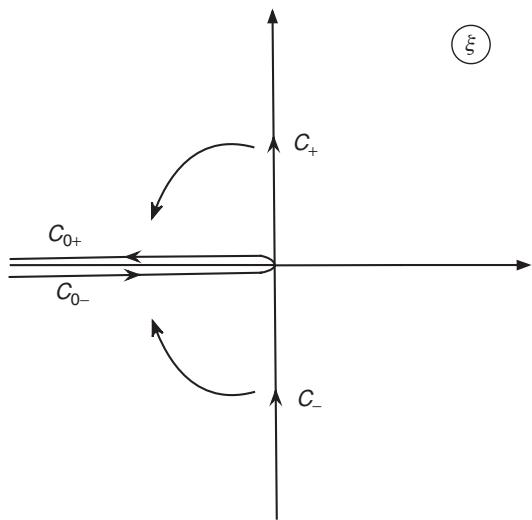
\includegraphics[width=0.5\textwidth]{figs/ch07/fig_7.5.jpg}
\caption*{图 7.5\quad 计算 $I_{1}$ 时在复 $\xi$ 平面中所用的积分围道。$C_{+}$ 是沿实轴闭合于上半平面的围道，$G^{\mathrm{R}}$ 在其上解析；同样，$C_{-}$ 闭合于下半平面，$G^{\mathrm{A}}$ 在其上解析。$C_{0-}$ 与 $C_{0+}$ 表示它们旋转 $90^{\circ}$ 后的围道，完全闭合于相对虚轴的左半平面内。}\label{fig:auto:7.5}
\end{figure}

\begin{align*}
I_{1} &= \frac{2\mathrm{i}}{(2\pi)^{d+1}}\int\mathrm{d}^{d}\mathbf{p}\int_{-\infty}^{0}\mathrm{d}\xi\,\frac{\mathrm{d}}{\mathrm{d}\xi}\ln\frac{G^{\mathrm{R}}(\xi,\mathbf{p})}{G^{*}_{\mathrm{R}}(\xi,\mathbf{p})} \\
&= -\frac{2}{\pi(2\pi)^{d}}\int\mathrm{d}^{d}\mathbf{p}\int_{-\infty}^{0}\mathrm{d}\xi\,\frac{\mathrm{d}}{\mathrm{d}\xi}\phi_{\mathrm{R}} \\
&= \frac{2}{(2\pi)^{d}}\int\mathrm{d}^{d}\mathbf{p}\,\frac{1}{\pi}\left[\phi_{\mathrm{R}}(-\infty) - \phi_{\mathrm{R}}(0)\right]
\tag{7.140}
\end{align*}
其中 $\phi_{\mathrm{R}}$ 是推迟格林函数的相位。在 $-\infty$ 处，$G^{\mathrm{R}}$ 为负实数。注意到推迟传播子的相位为 $\pi$，我们立即看到 $I_{1}$ 化为卢廷格定理。

那么 $I_{2}$ 呢？只要自能对 $\omega$ 是次线性的，$I_{2}$ 中的被积函数就可以分部积分。在许多情形下确实如此，于是 $I_{2}$ 通常化为
\begin{equation*}
I_{2} = 2\mathrm{i}\lim_{t \to 0^{+}}\int\frac{\mathrm{d}^{d}\mathbf{p}}{(2\pi)^{d}}\int\frac{\mathrm{d}\omega}{2\pi}\,\Sigma(\omega,\mathbf{p})\frac{\partial}{\partial\omega}\mathcal{G}(\omega,\mathbf{p})\,\mathrm{e}^{\mathrm{i}\omega t}.
\tag{7.141}
\end{equation*}
可以证明，这个积分在微扰论中逐阶为零（L1960）。论证十分简单：每一项都含有 $1/\omega$ 的更高次幂，因而从 $-\infty$ 到 $\infty$ 积分后为零。于是，我们就得到了前面宣称的结果：粒子密度由格林函数为正的那部分动量空间区域上的积分给出。卢廷格定理存在若干著名的例外，我们将在第 16 章中讨论。

\section*{习题}
\addcontentsline{toc}{section}{习题}

\textbf{习题 7.1}\quad 矩阵元 $V_{\mathbf{k}d}$ 计入了杂质上的电子与能带中电子之间的相互作用，它在用哈特里–福克方法确定杂质态与连续态时被略去。库仑矩阵元 $\langle\mathbf{k},\mathbf{k}'|V_{\mathrm{ee}}|d,\mathbf{k}'\rangle$ 对能带中其他电子 $k'$ 求和后，把一个电子从杂质能级搬到一个连续能级 $\mathbf{k}$ 上。试由这一残余库仑相互作用估计 $V_{\mathbf{k}d}$ 的大小。

\textbf{习题 7.2}\quad 试在安德森模型的哈特里–福克近似下，显式计算各个 $\epsilon_{n\sigma}$。

\textbf{习题 7.3}\quad 试显式证明：安德森哈密顿量的哈特里–福克近似可以写成式 (7.9) 的形式，其中 $a^{\dagger}_{n\sigma}$ 由式 (7.8) 定义。

\textbf{习题 7.4}\quad 试证明：当 $\epsilon_{d} = -U/2$ 时，安德森模型中的杂质项 $\sum_{\sigma}\left(\epsilon_{d}n_{d\sigma} + Un_{d\uparrow}n_{d\downarrow}\right)$ 在变换 $a^{\dagger}_{d} \leftrightarrow a_{d}$ 下不变。

\textbf{习题 7.5}\quad 考虑编时玻色格林函数
\begin{equation*}
G(\mathbf{r},t;\mathbf{r}',t') = -\mathrm{i}\langle T\psi(\mathbf{r},t)\psi^{\dagger}(\mathbf{r}',t')\rangle,
\tag{7.142}
\end{equation*}
以及玻色的超前与推迟格林函数。仿照费米格林函数推导中的相应步骤，计算它们的傅里叶变换。显式导出其实部与虚部之间的关系。特别地，你应当证明
\begin{equation*}
G^{\mathrm{R}}(\omega,\mathbf{p}) = \mathrm{Re}G(\omega,\mathbf{p}) + \mathrm{i}\tanh(\omega/2T)\mathrm{Im}G(\omega,\mathbf{p}).
\tag{7.143}
\end{equation*}
在 $G^{\mathrm{A}}$ 的类似表达式中，第二项带负号。

\section*{参考文献}
\addcontentsline{toc}{section}{参考文献}

\begin{itemize}[leftmargin=2em,itemsep=0pt,parsep=0pt,label={}]
\item [A1961] P. W. Anderson, Phys. Rev. 124, 41 (1961).
\item [BC1989] D. Baeriswyl and D. K. Campbell, eds. Interacting Electrons in Reduced Dimensions (Plenum Press, New York, 1989).
\item [D2003] I. Dzyaloshinskii, Phys. Rev. B 68, 85113/1-6 (2003).
\item [F1958] J. Friedel, Nuovo Cimento Suppl. VII, 287 (1958).
\item [GZ1974] G. Grüner and A. Zawadowski, Rep. Prog. Phys. 37, 1497 (1974).
\item [H1964] J. Hubbard, Proc. Roy. Soc. London A 276, 238 (1964).
\item [L1960] J. M. Luttinger, Phys. Rev. 119, 1153 (1960).
\item [M1955] T. Matsubara, Prog. Theor. Phys. 14, 351 (1955).
\item [M1960] B. T. Matthias, M. Peter, H. J. Williams, A. M. Clogston, E. Corenzwit, and R. C. Sherwood, Phys. Rev. Lett. 5, 542 (1960).
\item [S1938] E. C. Stoner, Proc. Roy. Soc. London A 165, 372 (1938).
\end{itemize}
